\section{Design}
HTPT is designed to be a SOCKS proxy. Since client and server HTTP traffic is different, the encoding in each direction is asymmetric. That is, the client-side and server-side encoding is different, and the decoding is similarly asymmetric such that the client can decode server data and vice versa. In what follows, the threat model will be discussed, followed by the goals, HTPT's architecture, and finally the implemented encoding schemes.

\subsection{Threat Model}
HTPT's threat model includes the following:
\begin{enumerate}
  \item Lightweight Deep Packet Inspection (DPI) is used. The DPI device may look at the header and contents of packets, but may not reassemble streams or otherwise retain state.
  \item Stateful DPI is not used frequently. This is due to the cost of remembering state information about a particular connection or series of connections.
  \item HTTP traffic is not widely blocked. Specific sites may be blocked but through an alternate mechanism (e.g., DNS redirection).
  \item Connection to a generic web server for a long period of time may be considered unusual, but connecting to an image server for a long period of time is less unusual.
  \item Image files transferred over HTTP can be verified to be valid images. Manual checking of image data will not happen due to cost.
\end{enumerate}

\subsection{Design Goals}
With the threat model in mind, the main goal is to increase the cost for a censor to discover the underlying Tor stream. For this reason, the Tor bridge will mimic an image gallery. Authenticated users will be allowed to send Tor traffic through the web server, while non-authenticated users will be returned a simple image gallery website. This means that the website must be able to correctly identify Tor and non-Tor traffic, and direct the traffic to the correct handlers. 

An additional goal is to provide plausible traffic going from the client to the server and vice versa. This effectively means that multiple encoding schemes must be created, as client traffic looks significantly different from server traffic in HTTP. 

In many situations, users will want to use HTTP to upload large amounts of data. However, HTTP and our transport are client-server protocols, which means clients typically send small requests to the server and the server returns large responses. HTPT mimics this structure, but also allows the user to achieve significant upload throughput. By structuring the upload traffic to look like images being uploaded to an image gallery, the user can achieve reasonable upload throughput while still maintaining an innocuous connection.

Preventing obvious fingerprintable behaviors is also a desired goal. This means that the server should not always send 128KB JPEGs, but rather it should vary the size and data type regularly.  

Reasonable performance, as measured by both `goodput' and latency, is a desired goal. Latency is most important for users of interactive websites, while reasonable goodput is required for uploading and downloading bulk data. 

\subsection{Motivations}
Though it seems odd to add yet another layer to an already tall stack, HTPT is similar to other protocols like IPSEC. It seems like the additional layer would introduce excessive overhead, but the purpose of this layer is to provide security first and performance second. This layer can be removed or inserted as necessary and is not required to exist. Despite the focus of this protocol on security, the size of images allow large amounts of data to be sent with limited headers.

\cite{Ref2} discusses the need to use the applications themselves and not just the protocol to obfuscate traffic. Otherwise adversaries can easily identify obfuscated traffic by finding differences in implementations of the protocols by the application and by the obfuscating layer. For example, Apache may implement a particular part of HTTP different from specification, while the obfuscating layer may not. This would make it susceptible to fingerprinting. As such, using actual applications for generating HTTP requests and responses will be necessary.

\subsection{Architecture}
The overall architecture is represented in Figure~\ref{fig:overall_arch}. It is a basic client-server model, but with several important additional layers.

\begin{figure}[t]
\centering
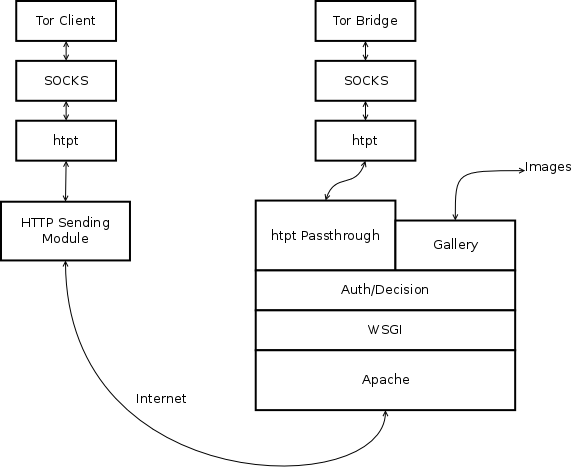
\includegraphics[width=0.7\textwidth]{Overall_architecture}
\caption{Overall Architecture}
\label{fig:overall_arch}
\end{figure}

On the client-side, there is a SOCKS interface that HTPT presents to its user, typically Tor as is represented here. HTPT is then connected to an HTTP sending module that interacts with the server-side.

The server-side from the top down is very similar: Tor connects via SOCKS with HTPT. At this point, the design diverges significantly. For this, looking from the bottom up is useful. 
%The client uses Selenium, a web browser orchestration framework, in conjunction with the Tor Browser Bundle, a packaged Tor client and Firefox web browser, to properly simulate web traffic and handle errors. 
The client uses Headless Webkit, which is the Webkit browser engine that has been modified to not need user interaction to properly simulate web traffic and handle errors.
The client connects to Apache, which is running the Web Server Gateway Interface module. This is a specification to allow web servers to communicate with web applications \cite{Ref16}. This is used to interface with the Authorization/Decision module that is part of the HTPT package. It is used to decide whether to send the traffic to the Image Gallery (for non-authorized traffic), or to the HTPT Passthrough (for authorized traffic). This is what it sounds: a simple passthrough. Traffic is then handed off the HTPT. 

The reverse is also true: traffic from the Tor Bridge to the Tor client goes through the same layers, just in reverse. 

\begin{figure}[b]
\centering
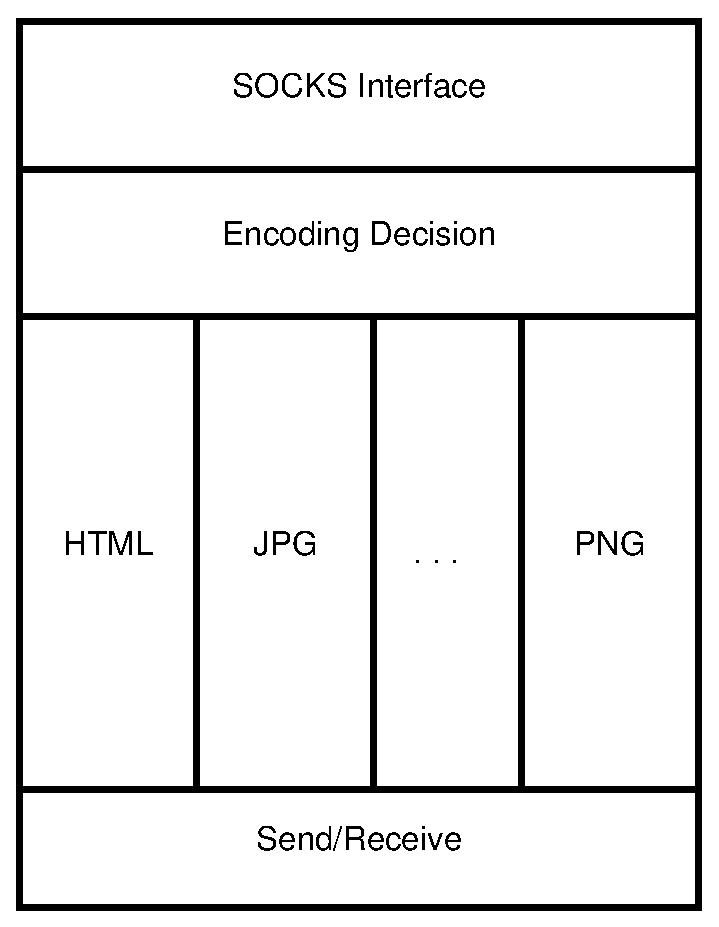
\includegraphics[width=0.3\textwidth]{htpt_architecture}
\caption{Modules within HTPT}
\label{fig:htpt_modules}
\end{figure}

Within HTPT, there are four main modules, as can be seen in Figure~\ref{fig:htpt_modules}. The SOCKS interface is the primary interface for communicating with Tor. This can also be used for other clients in a similar fashion, but in a much more limited manner.

The Encoding Decision module is the main location where anti-fingerprinting measures are taken. This module varies the encoding scheme and encoding amount such that the same style of data is not seen consistently. This is done by using a timer to buffer data up to a random amount of data to be sent. If that random amount is seen before the timer expires, it is sent, and a new random time and amount of data is chosen. This should make inter-arrival times more random than Tor normally is. 

Which encoding scheme is chosen depends on whether HTPT is acting in the client or server mode, and the data rate. This is measured based on the pervious transmission. That is, if 1000 bytes was received in the previous 10 milliseconds, the data rate can be calculated as being 100,000 bytes per second. This assumes that the data rate stays constant, which is why the time and buffer sizes are used in conjunction with each other.

This also acts as a framing module. Since each send operation opens a transient connection, reordering of data is vital. To handle this, sequence numbers are assigned by the Encoding Decision module. It is responsible for reorder of received data, for similar reasons. 

The Send/Receive module is an interface module. It is different for both the client and the server, as the lower interface is different. The client-side Send/Receive module will interface with an HTTP Sending Module, while the server-side will interface with the HTPT Passthrough.

Between the Send/Receive module and the Encoding Decision module lies the encoding modules themselves. They have a standard interface and are designed in such a way that new encoding modules can be added. For instance, if a developer wanted to create CSS encoder that generated CSS that encodes data, it could be added to the existing encoders.

Of note: this is a pull protocol. The client can push data to the server, but the server must be polled for more data. This is due to the nature of HTTP, and such mechanisms for polling for more data already exist: see how AJAX systems work.

\subsection{Encoding Schemes}
There are currently six developed encoding modules. Each takes in a common header, optionally appends its own header, and a quantity of data. This is then encoded and sent out. The header is retrieved from the Encoding Decision module, such that consistent sequence numbers can be retrieved. Local headers can consist of padding information, if the particular item sends fixed-width data chunks. 

\begin{enumerate}
  \item \emph{Advertising URL Encoder} --- This encodes 40 bytes of data at a time by mimicking an advertising header. These frequently have 80-character hex-encoded identifiers contained within them, and are useful for encoding small amounts of data from the client to the server.
  \item \emph{Google Search String Encoder} --- This encodes variable amounts of data, albeit small amounts of data. Initial implementation uses 16 common English words to represent 4-bits of data, effectively acting as a hex encoder. These are then places in what looks like a Google search string that can be decoded on the receiving end.
  \item \emph{Baidu Search String Encoder} --- This is a similar scheme as the Google Search String Encoder, except that it is designed to create Baidu-like search strings.
  \item \emph{BMP Encoder} --- This is the most basic image encoder. A valid bitmap header is created, then the raw data makes up the image data.
  \item \emph{JPEG Encoder} --- By using lossless JPEGs, data can be sent across without loss. This uses the BMP Encoder, and converts it into a lossless JPEG to be sent by either the client or server.
  \item \emph{PNG Encoder} --- This is a similar scheme as the JPEG Encoder, with PNGs as output.
\end{enumerate}

\subsection{Framing and Performance Implications}
As noted above, the encoding is an encapsulation scheme. The data from Tor, or any other SOCKS enabled client, is treated as a byte-stream, much like data that is sent via TCP. A 4-byte header is attached on each segment sent. The segment is then wrapped based on the encoding scheme, which is where the overhead comes into play.


TODO: NEED A DIAGRAM OF HEADER


As one of the design goals is to have reasonable goodput performance, the overhead must be discussed. 


TODO: NEED A TABLE OF OVERHEAD RATIOS, MINIMUM AND MAXIMUM, number of bytes of overhead per item.
